% Copyright 2004 by Till Tantau <tantau@users.sourceforge.net>.
%
% In principle, this file can be redistributed and/or modified under
% the terms of the GNU Public License, version 2.
%
% However, this file is supposed to be a template to be modified
% for your own needs. For this reason, if you use this file as a
% template and not specifically distribute it as part of a another
% package/program, I grant the extra permission to freely copy and
% modify this file as you see fit and even to delete this copyright
% notice. 

\documentclass{beamer}

\usepackage{epstopdf}
\graphicspath{{figures/}} % Location of the graphics files
\newcommand{\abnet}{{\sc ABnet}}


% There are many different themes available for Beamer. A comprehensive
% list with examples is given here:
% http://deic.uab.es/~iblanes/beamer_gallery/index_by_theme.html
% You can uncomment the themes below if you would like to use a different
% one:
%\usetheme{AnnArbor}
%\usetheme{Antibes}
%\usetheme{Bergen}
%\usetheme{Berkeley}
%\usetheme{Berlin}
%\usetheme{Boadilla}
%\usetheme{boxes}
%\usetheme{CambridgeUS}
%\usetheme{Copenhagen}
%\usetheme{Darmstadt}
%\usetheme{default}
%\usetheme{Frankfurt}
%\usetheme{Goettingen}
%\usetheme{Hannover}
%\usetheme{Ilmenau}
%\usetheme{JuanLesPins}
%\usetheme{Luebeck}
\usetheme{Madrid}
%\usetheme{Malmoe}
%\usetheme{Marburg}
%\usetheme{Montpellier}
%\usetheme{PaloAlto}
%\usetheme{Pittsburgh}
%\usetheme{Rochester}
%\usetheme{Singapore}
%\usetheme{Szeged}
%\usetheme{Warsaw}

\title[Hybrid STD-DNN system]{
Hybrid Spoken Term Discovery-DNN System
}

% A subtitle is optional and this may be deleted
\subtitle{Finding words to learn segments}

\author[Roland Thiolliere]{
Roland Thiolli\`ere\inst{*}, Ewan Dunbar\inst{*}, Gabriel Synnaeve\inst{*\dagger}\\Maarten Versteegh\inst{*}, Emmanuel Dupoux\inst{*}
}
% - Give the names in the same order as the appear in the paper.
% - Use the \inst{?} command only if the authors have different
%   affiliation.

\institute[ENS] % (optional, but mostly needed)
{
\inst{*} LSCP, \'{E}cole Normale Sup\'{e}rieure / EHESS / CNRS, Paris, France\\%[0.3ex]
\inst{\dagger} now at Facebook AI Research\\[0.5ex]
\inst{} \begin{small}\texttt{rolthiolliere@gmail.com, emd@umd.edu, gabrielsynnaeve@gmail.com, maartenversteegh@gmail.com, emmanuel.dupoux@gmail.com}\end{small}
}
% - Use the \inst command only if there are several affiliations.
% - Keep it simple, no one is interested in your street address.

\date{Interspeech, 2015}
% - Either use conference name or its abbreviation.
% - Not really informative to the audience, more for people (including
%   yourself) who are reading the slides online

%\subject{Theoretical Computer Science}
% This is only inserted into the PDF information catalog. Can be left
% out. 

% If you have a file called "university-logo-filename.xxx", where xxx
% is a graphic format that can be processed by latex or pdflatex,
% resp., then you can add a logo as follows:

% \pgfdeclareimage[height=0.5cm]{ENS-logo}{ENS_LOGO}
% \logo{\pgfuseimage{ENS-logo}}

% Delete this, if you do not want the table of contents to pop up at
% the beginning of each subsection:
% \AtBeginSubsection[]
% {
%   \begin{frame}<beamer>{Outline}
%     \tableofcontents[currentsection,currentsubsection]
%   \end{frame}
% }

% Let's get started
\begin{document}

\begin{frame}
  \titlepage
  
\includegraphics[width=1cm]{CNRS_LOGO.eps}
  \hfill
  
\includegraphics[width=0.9cm]{EHESS_LOGO}
  \hfill
  
\includegraphics[width=0.8cm]{ENS_LOGO}
  \hfill
  
\includegraphics[width=1cm]{ERC_LOGO}
  \hfill
  
\includegraphics[width=1.2cm]{PSL_LOGO}


\end{frame}

% \begin{frame}{Outline}
%   \tableofcontents
%   % You might wish to add the option [pausesections]
% \end{frame}

% Section and subsections will appear in the presentation overview
% and table of contents.
\section{Finding words to learn phonemes}

\subsection{System overview and results}

\begin{frame}{Finding words to learn phonemes}{System overview and results}
  \begin{itemize}
  \item {
    Use Track 2 to help with Track 1.
  }
  \item {
    Two components: spoken term discovery and siamese deep neural network.
  }
  \end{itemize}
\begin{figure}
  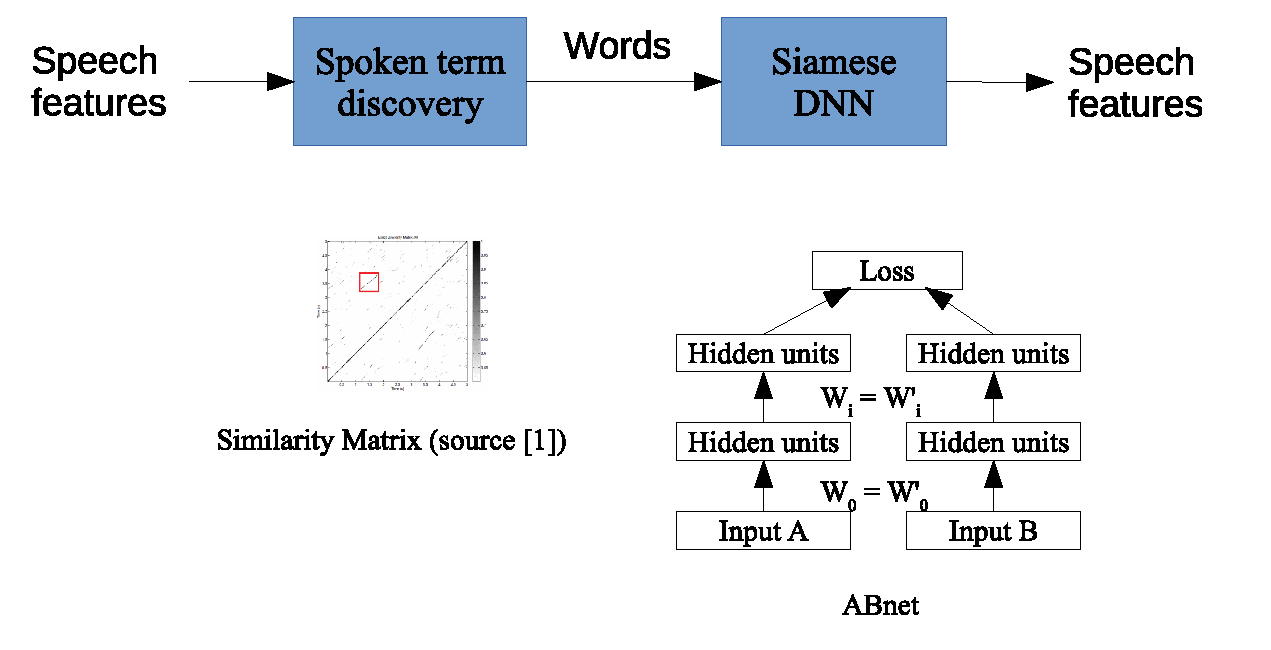
\includegraphics[width=0.7\textwidth]{system_presentation.eps}
\end{figure}

\tiny
[1] A. Jansen and B. van Durme, “Efficient spoken term discovery using
randomized algorithms,” in Proceedings of ASRU, 2011
% \nocite{*} % Print all references regardless of whether they were cited in the poster or not
% \bibliographystyle{IEEEtran} % Plain referencing style
% \bibliography{bib} % Use the example bibliography file sample.bib

\end{frame}

% % Placing a * after \section means it will not show in the
% % outline or table of contents.
% \section*{Summary}

\begin{frame}{Track 1 evaluation: ABX}
  \begin{itemize}
  \item {
      Improved over baseline a lot.
  }
  \item {
    Close to topline in english!
  }
  \end{itemize}
\begin{figure}
  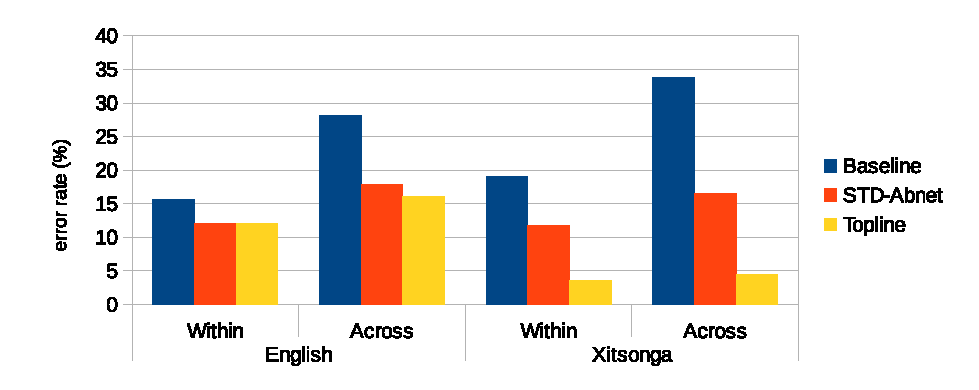
\includegraphics[width=0.9\textwidth]{results.eps}
  \caption{ Within and across speaker Minimal Pair ABX error rates}
\end{figure}
\end{frame}

% \begin{frame}{Summary}
%   \begin{itemize}
%   \item
%     The \alert{first main message} of your talk in one or two lines.
%   \item
%     The \alert{second main message} of your talk in one or two lines.
%   \item
%     Perhaps a \alert{third message}, but not more than that.
%   \end{itemize}
  
%   \begin{itemize}
%   \item
%     Outlook
%     \begin{itemize}
%     \item
%       Something you haven't solved.
%     \item
%       Something else you haven't solved.
%     \end{itemize}
%   \end{itemize}
% \end{frame}



% All of the following is optional and typically not needed. 
% \appendix
% \section<presentation>*{\appendixname}
% \subsection<presentation>*{For Further Reading}

% \begin{frame}[allowframebreaks]
%   \frametitle<presentation>{For Further Reading}
    
%   \begin{thebibliography}{10}
    
%   \beamertemplatebookbibitems
%   % Start with overview books.

%   \bibitem{Author1990}
%     A.~Author.
%     \newblock {\em Handbook of Everything}.
%     \newblock Some Press, 1990.
 
    
%   \beamertemplatearticlebibitems
%   % Followed by interesting articles. Keep the list short. 

%   \bibitem{Someone2000}
%     S.~Someone.
%     \newblock On this and that.
%     \newblock {\em Journal of This and That}, 2(1):50--100,
%     2000.
%   \end{thebibliography}
% \end{frame}

\end{document}


